\section{Wireless Networks}
\begin{tabular}{|l|l|l|}
	\hline
	\textbf{Typ} & \textbf{Beschreibung} & \textbf{Standarts}\\
	\hline
	PAN & Personal Area Network & Bluetooth, ZigBee, Ultrawideband\\
	\hline
	WLAN & Wireless Local Area Network & WLAN, Wi-Fi\\
	\hline
	MAN & Metropolitan Area Network & WiMAX\\
	\hline
	WWAN & Wireless Wide Area Network & GPRS, EDGE, UMTS, LTE\\
	\hline
\end{tabular}
\subsection{PAN - Personal Area Networks \formelbuch{264}}
\begin{tabular}{|l|l|l|l|l|l|l|} \hline
name of system & RF & b/w per channel & data rate  & tx power	& distance  & modulation  \\
\hline \hline
Bluetooth 802.15.1 & 2.4\,GHz	& 1\,MHz	& 1\,Mbit/s	      & 100\,mW	 & 80\,m	& GFSK \\ \hline
ZigBee 802.15.4	   & 868\,MHz,& 2\,MHz	& 20\,kbit/s,     & 100\,mW  & 75\,m	& BPSK, \\
              	   & 915\,MHz,& 2\,MHz	& 40\,kbit/s,     & 100\,mW  & 75\,m	& BPSK,  \\
                   & 2.4\,GHz & 2\,MHz	& 250\,kbit/s     & 100\,mW  & 75\,m	& O-QPSK \\ \hline
DECT	             & 1.9\,GHz	& 1.728\,MHz & 1152\,kbit/s	& 100\,mW	 & 300\,m	& GFSK \\ \hline
\end{tabular}\\

\textbf{Bluetooth \formelbuch{264}}\\
\textbf{ZigBee \formelbuch{264}}\\
\textbf{Ultrawideband (UWB)\formelbuch{265}}

\subsection{WLAN - Wireless Local Area Networks}
Wi-Fi is defined as any wireless local area network (WLAN) products that are based on the Institute of Electrical and Electronics Engineers' (IEEE) 802.11 standards. \\

\begin{tabular}{|l|l|p{3cm}|p{3cm}|l|l|} \hline
Technology & Spectrum & Max. Bandwidth & Modulation & MIMO streams & Max Data Rate
\\ \hline \hline
802.11  & 2.4\,GHz  & 22 MHz           & FHSS, DSSS  & n.a. & 1-2\,Mbps  \\ \hline
802.11a    &   5\,GHz  & 20 MHz           & OFDM      & n.a. & 54\,Mbps \\ \hline
802.11b    & 2.4\,GHz  & 22 MHz          & DSSS     & n.a. & 11\,Mbps \\ \hline
802.11g    & 2.4\,GHz  & 20 MHz           & OFDM, DSSS   & n.a.  & 54\,Mbps \\ \hline
802.11n   & 2.4 \& 5\,GHz & 20 or 40 MHz	     & OFDM  & 4 & 65-300\,Mbps \\ \hline
802.11ac   &   5\,GHz  & 20 - 160 MHz 	  & OFDM	& 8 & 86-780\,Mbps \\ \hline
\end{tabular}

\subsubsection{MAC Layer}
WiFi uses Carrier Sense Multiple Access (CSMA) on the MAC Layer. The station ready to send data starts sensing the medium and 
if the medium is free for the duration of a DIFS, the station can start sending directly. If the medium is busy, the station has to 
wait for a free DIFS and additionally wait a random back-off time (collision avoidance, multiple of slot-time of 20us). In case 
another station occupies the medium during the backoff time waiting, the backoff counter stops at the current value and continue
decreasing from that value at the next round (fairness). 

With the first transmission attempt the random slot for the backoff-procedure is chosen between 0 - $CW_{min}$, where $CW_{min}$ for 11b and g is 31, for 11n it's 15. \\
On any further attempt the random slot is chosen between 0 - 63, then 0 - 127, ... 0 - $CW_{max}$. \\
$CW_{max}=1023$ slots (20 ms), afterwards the frame is discarded on the MAC Layer. \\

\begin{tabular}{ll}
	\parbox{7cm}{
		\textbf{Example:} \\
		\begin{itemize}	
			\item  no RTS- and CTS-packet are used
			\item  DIFS = 50 us, SIFS = 10 us and a slot time = 20 us
			\item  the transmission period for each data packet is 500 us
			\item  the transmission period for each ACK-packet is 140 us
			\item  STA1 has a data packet pending and a remaining backoff of 20 slots
			\item  STA2 has a data packet pending and a remaining backoff of 5 slots
			\item  STA3 gets a request to send a packet from a higher layer at t = 750 us
			and chooses a random backoff of 10 slots
		\end{itemize}
	}
	& \parbox{11cm}{
		\fbox{ 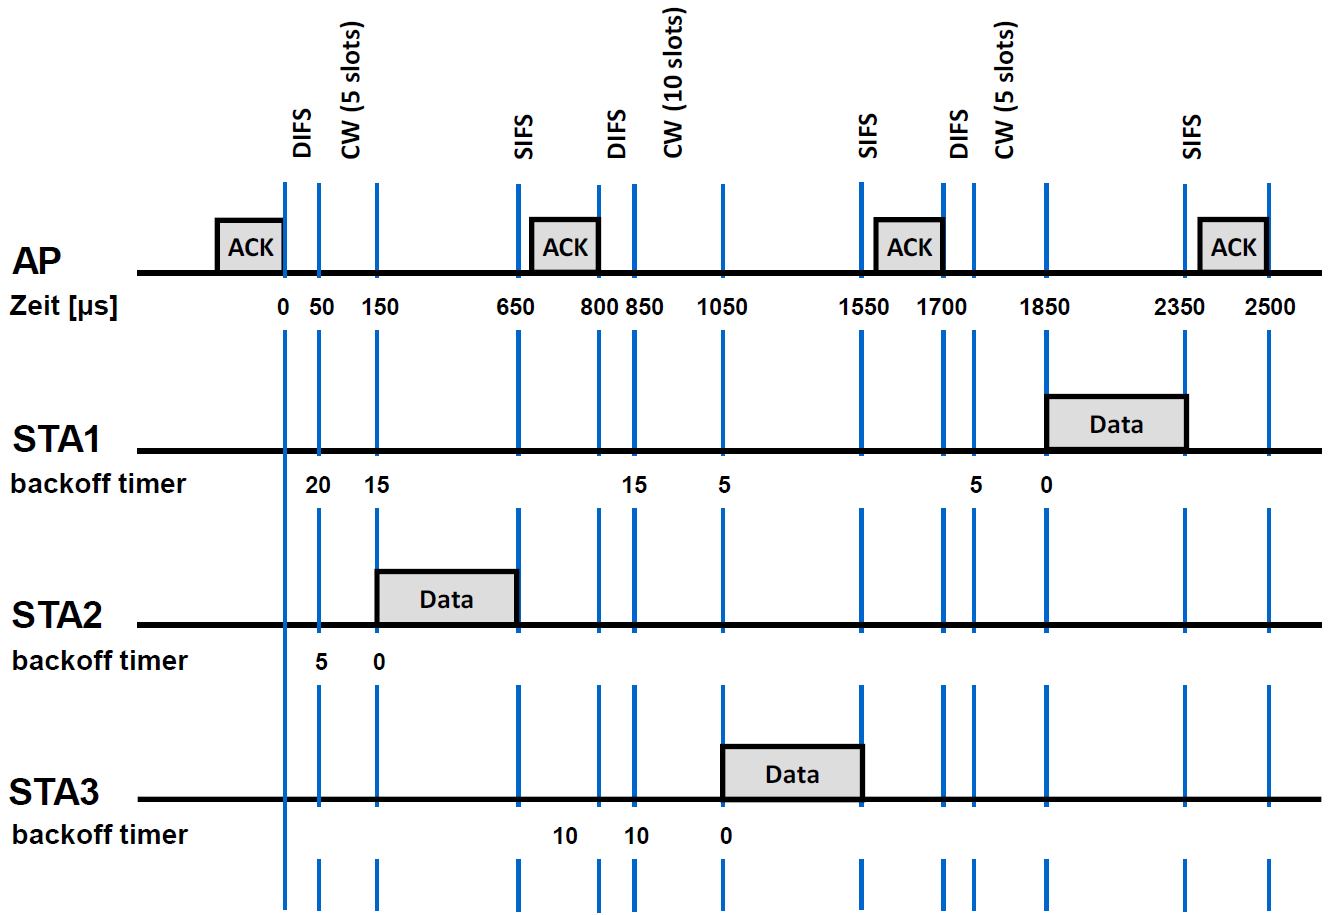
\includegraphics[width=11cm]{./bilder/wlan-csma.png}} \\ 
	}
\end{tabular}	
	
\subsubsection{PHY Layer of IEEE 802.11g}
	\begin{tabular}{ll}
		\parbox{11cm}{
			For the PHY Layer of 802.11g standard OFDM with 52 subchannels is used (4 pilot channels and 48 data channels). 
			The symbol rate is 250 kSps and therefore the symbol period is $T_{symbol}=4\mu$s. The 11g standard defines several modulation
			and coding schemes with different data rates. Which one of these can be used depends on the actual SNR
			(the higher the SNR, the higher the modulation). 				
		}
		& \parbox{7cm}{
			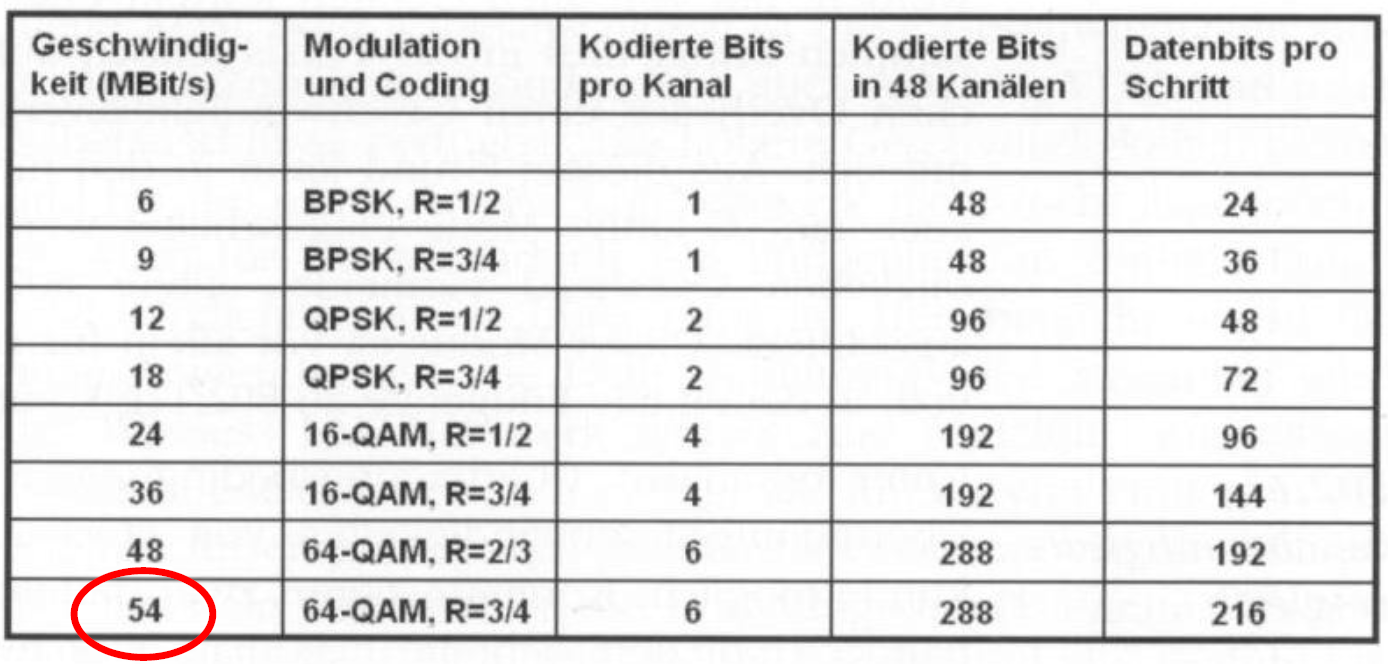
\includegraphics[width=7cm]{./bilder/wlan-phy.png} \\ 
		}
	\end{tabular}
	
	The data rate R is calculated as follows: $R=\frac{N_{OFDM}\cdot BPC}{T_{symbol}}\cdot R_{FEC}$ \\
	Where $N_{OFDM}=$Number of OFDM data channels $=48$ , $BPC=$Bits per channel , $R_{FEC}=$Coding rate \\
	
	Some 802.11g or 11a devices might have two Antennas. However, this is not intended for MIMO but rather
	for Antenna Diversity, i.e. improve the received signal by reducing the probability of deep fading. 

	In some cases there is the possibility to activate the option "G only". By doing so, the backwards
	compatibility with 11b devices is deactivated, but due to less interworking overhead the performance
	increases of about 40\%.
	
\subsection{MAN - Metropolitan Area Networks}
